% This is "sig-alternate.tex" V2.0 May 2012 This file should be compiled
% with V2.5 of "sig-alternate.cls" May 2012
% 
\documentclass[11pt]{article}
\usepackage{enumerate}
\usepackage{hyperref} 
\usepackage{url}
\usepackage{graphicx}
\usepackage{float}
\usepackage{placeins}
\graphicspath{{images/}}


\title{Reliable Multicast in the DETER network}
\author{
Vineet Ghatge & Anuj Gupta
}

\begin{document}

\maketitle

\section{Introduction}
\label{sec:intro}
The DETER testbed~\cite{Peterson} is shared infrastructure designed for medium-scale repeatable experiments in the domain of computer security. The testbed provides unique resources and a focus of activity for an open community of academic, industry, and government researchers working toward better defenses against malicious attacks on the world's networking infrastructure.

The DETER testbed~\cite{Peterson} is made up of several nodes, switches, and routers that can be configured to create a specified topology. The experiment nodes are connected to two networks at all times; an isolated experiment network which is used to conduct the experiment and a control network that can be used to send control signals and collect measurements during the experiment. The control network has multicast support to send and receive messages from several nodes at once. 

As Multicast~\cite{Intro} is UDP (User Datagram Protocol) based, it does not guarantee the delivery of a message stream. So the challenges faced by multicast are that the messages may be dropped, delivered multiple times , or delivered out of order. Our preliminary multicast experiments indicate that multicast network in DETER is unreliable. We aim at adding reliability mechanism to multicasting on DETER network to analyze its effect on the number of messages lost, size of the loss bursts and frequency of losses.

The current state of the art in DETER does not have any flexible and easy to use tools to measure the multicast loss bursts~\cite{DETER}. There have been several attempts in the past to emulate multicast in DETER, to the best of our knowledge we do not know if any of them have been successful so far. Our long term goals are 
\begin{enumerate}
\item Understand and evaluate the performance of multicast network on DETER for varying combinations.
\item Implementing reliability in the network and attempting to study the impact of size, frequency and factors affecting loss burst for multicast networks.
\end{enumerate}
This report presents an inital understanding of the DETER performance with respect to multicasting~\cite{PGM}~\cite{SRM}.

\section{Methodology} 
\label{sec:approach}
Multicast is a network addressing method for the delivery of information to a group of destinations simultaneously using the most efficient strategy to deliver the messages over each link of the network only once, creating copies only when the links to the multiple destinations split (typically at network switches and routers). A reliable multicast protocol adds the ability for receivers to detect lost and/or out-of-order messages and take corrective action (similar in principle to TCP), resulting in a gap-free, in-order message stream~\cite{Code}.

We will attempt to analyze experiment and control networks in DETER for the number of messages lost, size of the loss bursts and frequency of losses. Upon observing the unreliable behavior of both the networks, we will now add a simplistic reliability mechanism to multicasting in DETER lab. We will firstly attempt to add this mechanism for a one to one multicast network and then scale it up for a one to many multicast network. We will attempt to analyze its impact on performance, the size of the loss bursts and delay of the multicast messages.

Initally, the experiment is setup such that we have single sender and single receciver on the experimental network. The nodes have two NIC cards each of which are connected to the experiment and control network. We do not enforce any traffic shapping factors or parameters on the network, this ensures that no other parameters is going to affect the traffic flow across the link. We consider the following paramters to be crucial in affecting the network. 
\begin{enumerate}
\item \itemit{Burst Size}: This is defined as number of packets which are sent by the sender.
\item \itemit{Packet Size}: This is defined as the number of bytes per packet that are transmitted by the sender.
\item \itemit{Reciever Size}: This is defined as the number of recievers in the network.
\end{enumerate}
At each iteration of the burst size we evaluate loss burst, in order to facilitate and identify this: we construct a simple multicast packet which has a header of \itemit{12} bytes in size without the payload. One of the "fairly" missing factors of UDP is the absence of sequence numbers. The reason we call this fairly is contrasting behaviours of TCP versus UDP, one would notice this one of the features which is characteristic of a connection oriented protocol~\cite{Code}. We collect extensives amount of measurements such as - Sequence Number both at the sender and receiver, Nestat and Ethtools output. The latter two are required to monitor queues for any packet drops. Our Experiment is evaluated against both the control and experiment network. One would ideally expect the experiment network to perform better than control network. The experiment network is a more controlled environment, the link loss and bandwidth is configurable unlike the control network. The realibility of the 100Mbps link is not really controllable.{Need to add a diagram}

The multicast sender and receiver applications were written in C using the concept of Socket Programming API~\cite{Code}.To gather accurate data, we need to perform significant number of executions of our experiment and hence we wrote automation scripts. We wrote the following types of scripts –
\begin{enumerate}
\item \itemit{Shell scripts} : To evaluate missing sequence numbers based on the intersection of sender and reciver trace files~\cite{Ethtool,Netstat}.
\item \itemit{Gnuplot scripts} : Takes the sequence number of lost packets to plot the histograms~\cite{Gnuplot}.
\item \itemit{TCL scripts} : To enable workflow deterministic control when we scale the number of receviers and senders~\cite{Magi}.
\end{enumerate}
Since UDP has no deterministic information to inform the receivers about the number of packets being sent we introduce the concept of round number. We define one round from first packet to last packet sent from the sender for a fixed burst size. The round number is field defined as part of packet header. We perform a linear increment in burst size for a fixed size in every execution of the experiment. The sequence numbers generated are serially increasing till the end of each round. An end of round is indicated by a conflicting packet round number as opposed to a expected packet number at receivers end.

We scale the experiment to include the more number of receivers for a single source sender. We analyze the loss burst at each reciever to understand the dynamics of the packet loss. We vary the type of nodes being used. The nodes used are - bpc3000, pc3000 and bpc 2133, pc 2133. 
We conduct these experiments on emulab - an inital educational version of deterlab as well to holostically complete our analysis.{Need to add diagram & Code Snippet} 
 

\section{Results}
\label{sec:evaluation}
The experiment is conducted in two scenarios with the custom UDP packets constructed exclusively for experiments~\cite{DETER}.
\begin{enumerate}
\item \itemit{Experiment Network} : We deployed the application to create a socket on one of the internal IP address - 10.1.1.X. We exchanged traffic across the link and evaluated the loss burst.
\item \itemit{Control Network} : We deployed the application to create a aocket on one of the external IP address - 192.168.X.X. The path taken by this mode need not be an immediate hop. Based on the different combinations of packet size and burst size, we generate ten simulations. The average of these simulations gives us good overview and consistency of the network behaviours. We study each of these keeping one parameter constant at time.
\end{enumerate}

\subsection{Packet Size} 
In this section we keep the packet size constant(in our case its about 72 bytes), and vary the burst size of 100 and incrementally build it by factor 100 to understand its small scale jumps. We evaluate the network behaviour till about 5000 packets on both experiment and control mode.
Fig 1 shows behaviour of packet loss with varying burst size. We see that loss burst increments in a linear fashion. This behaviour is as expected. Loss rate is indicated by the averages accounted at every loss burst size(green line in the figures). Fig 3 is a plot in the similar lines as Fig 1, with burst size ranging between 1500-5000. The range between 4000 - 5000 in Fig 4 need some explanation as the loss reaches a constant change. This might be because of the devices being optmized for certain range values. We suspect this behaviour might continue and is an area to explore and understand.
\begin{figure}[!ht]
\centering
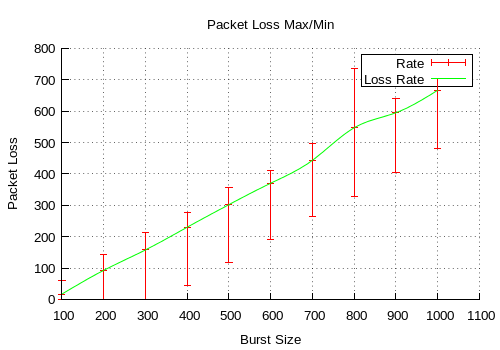
\includegraphics[width=0.8\textwidth]{Fig1.png}
\caption{Packet Loss on Control Network for Burst Size varying between 100-1000}
\end{figure}
\FloatBarrier
\begin{figure}[!ht]
\centering
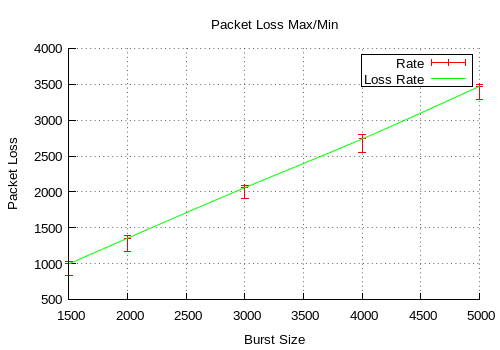
\includegraphics[width=0.8\textwidth]{Fig2.png}
\caption{Packet Loss on Control Network for Burst Size varying between 1500-5000}
\end{figure}
\FloatBarrier
\begin{figure}[!ht]
\centering
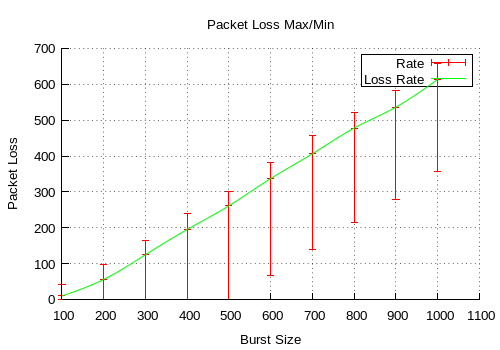
\includegraphics[width=0.8\textwidth]{Fig3.png}
\caption{Packet Loss on Experiment Network for Burst Size varying between 100-1500}
\end{figure}
\FloatBarrier
\begin{figure}[!ht]
\centering
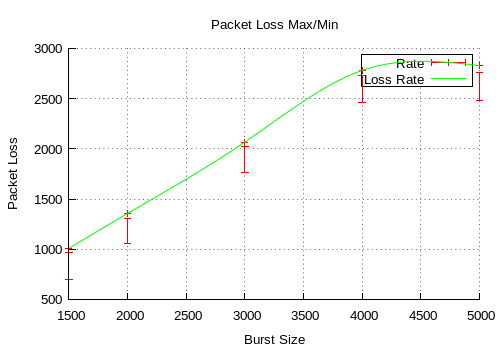
\includegraphics[width=0.8\textwidth]{Fig4.png}
\caption{Packet Loss on Experiment Network for Burst Size varying between 1500-5000}
\end{figure}
\FloatBarrier
Contrasting the control network versus experiment network, it is evident that control network is far more decremental in loss burst. This is indicated by the range of error bars which progressively shrink with packet size.
\subsection{Burst Size}
In this section we keep the burst size constant(same as above 5000 packets) and vary the packet size from 72 bytes upto 1212 bytes. We evaluate the network behaviour for both control and network mode. Notice, the comparison between Fig 5 - Fig 9, we do not see any loss burst till we reach above 100 packets. On average the loss burst varies from 40 to 100 packets for packet size between 72 bytes to 512 bytes.The losses are fairly consistent with progress of traffic in the control network.
\begin{figure}[!ht]
\centering
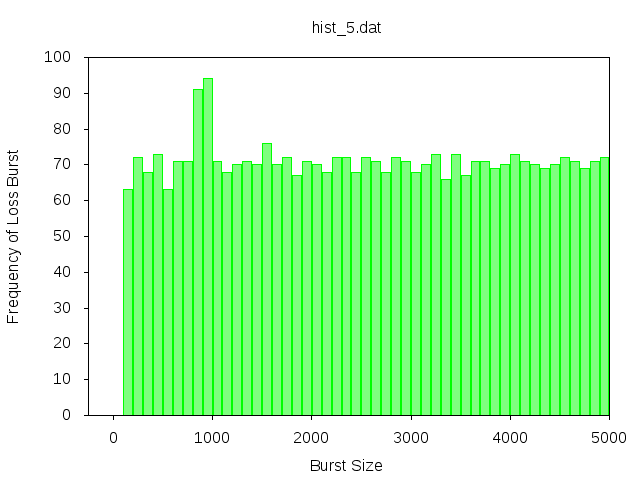
\includegraphics[width=0.8\textwidth]{seq50.png}
\caption{Frequency of Loss Burst on Control Network for 72 bytes and Burst Size of 5000 packets}
\end{figure}
\FloatBarrier
\begin{figure}[!ht]
\centering
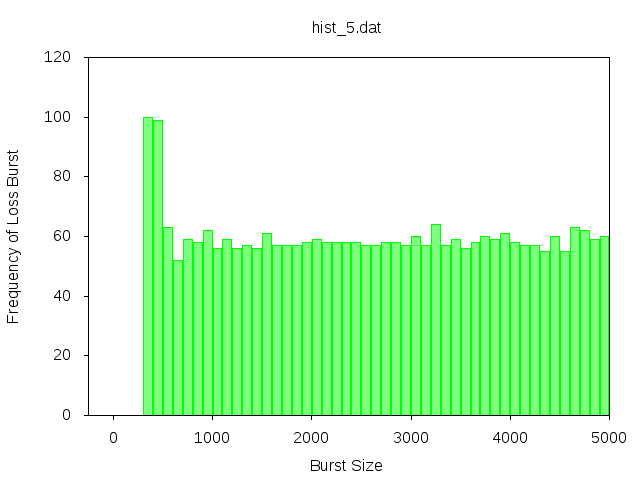
\includegraphics[width=0.8\textwidth]{seq100.png}
\caption{Frequency of Loss Burst on Control Network for 112 bytes and Burst Size of 5000 packets}
\end{figure}
\FloatBarrier
\begin{figure}[!ht]
\centering
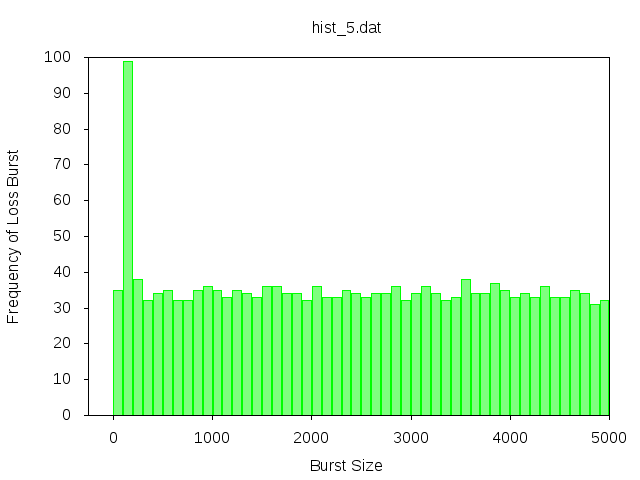
\includegraphics[width=0.8\textwidth]{seq500.png}
\caption{Frequency of Loss Burst on Control Network for 512 bytes and Burst Size of 5000 packets}
\end{figure}
\FloatBarrier
In theory, extrapolating our results we expect the loss burst to worsen or stay consistent with packet size increase. However, our results from Fig 8 - Fig 9 show that loss burst diminishes. One of the reasons why we might be seeing this behaviour is due to the optimization of the switches on the network. Our results from experiment network show the similar behaviour, however the loss percentage are far lesser than control network.
\begin{figure}[!ht]
\centering
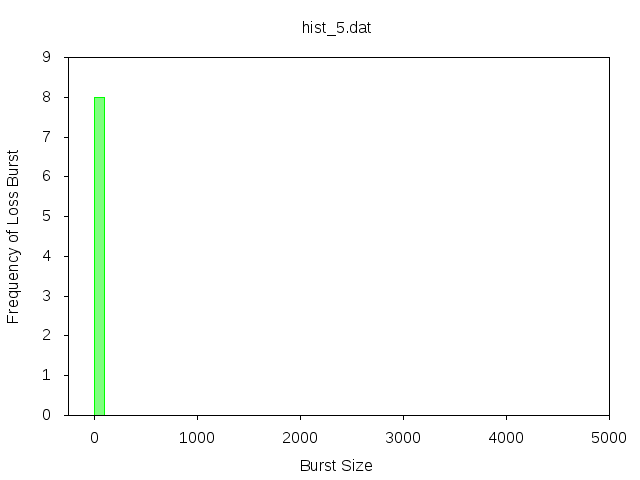
\includegraphics[width=0.8\textwidth]{seq1000.png}
\caption{Frequency of Loss Burst on Control Network for 1012 bytes and Burst Size of 5000 packets}
\end{figure}
\FloatBarrier
\begin{figure}[!ht]
\centering
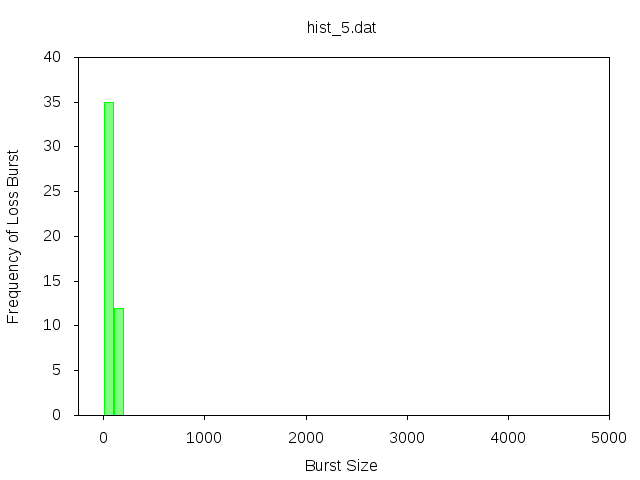
\includegraphics[width=0.8\textwidth]{seq1200.png}
\caption{Frequency of Loss Burst on Control Network for 1212 bytes and Burst Size of 5000 packets}
\end{figure}
\FloatBarrier
Our last graphs - Fig 10 and Fig 11 are 3D plot of data from all the experiments conducted. Notice the peak points in both the graphs which are indicative of "sweet" spots - point where the network has high degree of loss and this surge flattens out. These graphs have provided us useful data points in understanding how DETER behaves with multicast. Contrasting the two graphs - the control network degrades exponentially unlike the experiment network. Based on our analysis on DETER, we extended our experiment on Emulab. Our inital results suggest degraded performance, while we do not present the analysis here. The comparison might prove an useful baseline in understanding performance on DETER.
\begin{figure}[!ht]
\centering
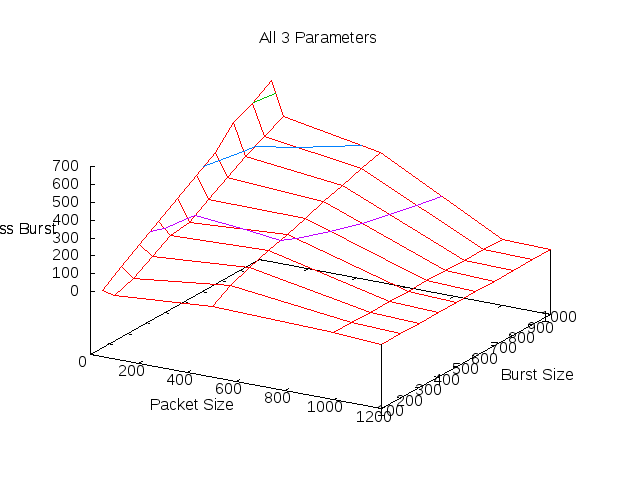
\includegraphics[width=0.8\textwidth]{control.png}
\caption{3D variation for Control Network - Deterlab}
\end{figure}
\FloatBarrier
\begin{figure}[!ht]
\centering
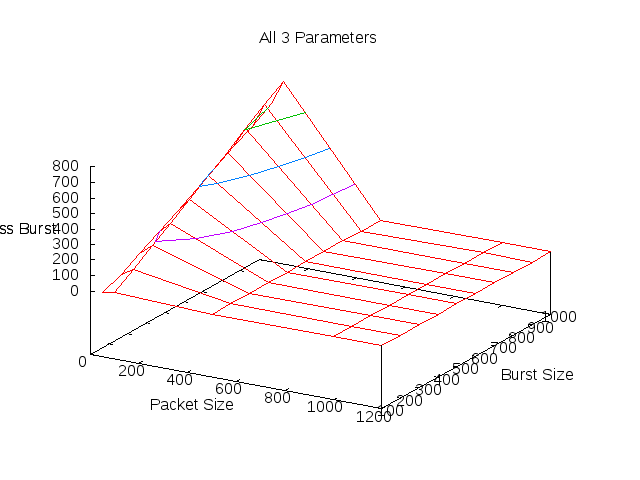
\includegraphics[width=0.8\textwidth]{exp.png}
\caption{3D variation for Experiment Network - Deterlab}
\end{figure}
\FloatBarrier

\subsection{Reciever Size}
We scale the number of reciever from one to about five and ten for the expermient network, we notice that the for same reciver multiple runs result in different behaviour in losses.{Need to write about 10 node size}
\begin{figure}[!ht]
\centering
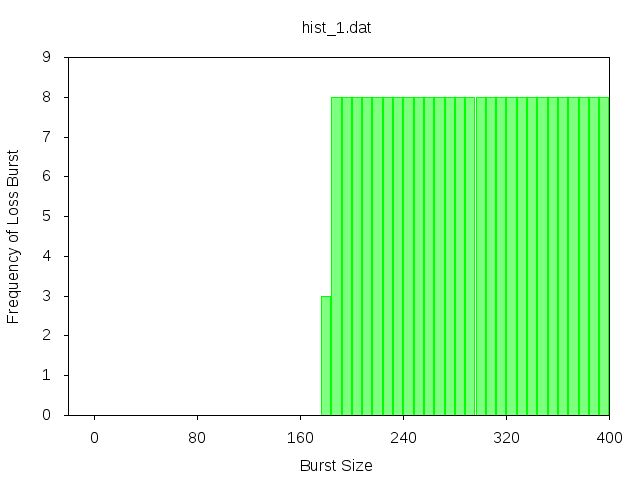
\includegraphics[width=0.8\textwidth]{Recv21.png}
\caption{Frequency of Loss Burst on Experiment Network for 112 bytes and Burst Size of 400 packets for Run 1 - Reciver 2}
\end{figure}
\FloatBarrier
\begin{figure}[!ht]
\centering
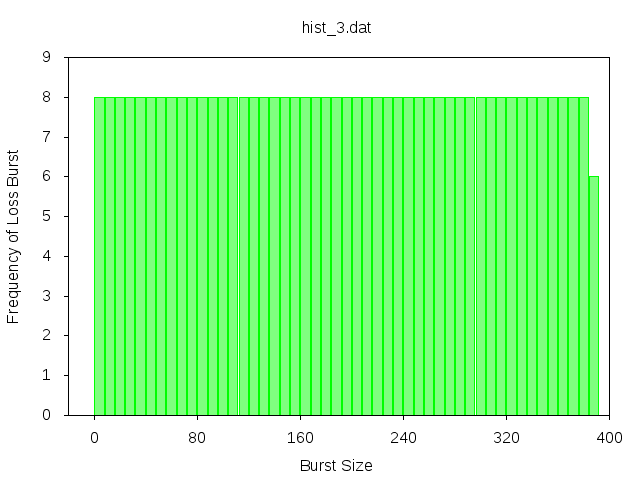
\includegraphics[width=0.8\textwidth]{Recv23.png}
\caption{Frequency of Loss Burst on Experiment Network for 112 bytes and Burst Size of 400 packets for Run 3 - Reciver 2}
\end{figure}
\FloatBarrier

\subsection{Emulab}
Emulab behaves better than deterlab for pc3000 nodes but not for pc850 node{Need to add more about the how, why about emulab}
\begin{figure}[!ht]
\centering
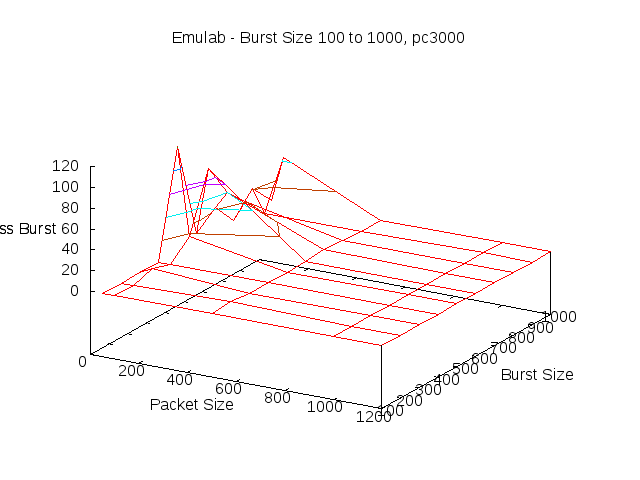
\includegraphics[width=0.8\textwidth]{3Demulab.png}
\caption{3D variation for Control Network - Emulab}
\end{figure}
\FloatBarrier
\begin{figure}[!ht]
\centering
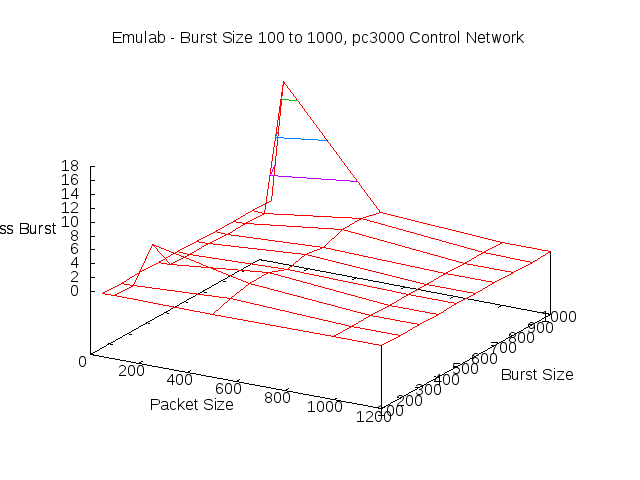
\includegraphics[width=0.8\textwidth]{3Demulab2.png}
\caption{3D variation for Control Network - Emulab}
\end{figure}
\FloatBarrier
\begin{figure}[!ht]
\centering
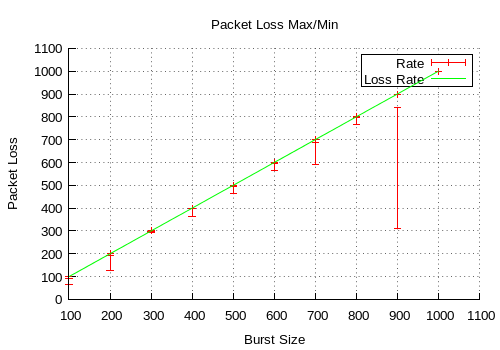
\includegraphics[width=0.8\textwidth]{EM.png}
\caption{Packet Loss in Emulab for bp850 for experiment network}
\end{figure}
\FloatBarrier
{Need to conduct for varying packet size and then plot 3d graph and also a plot for emulab control}

\section{Summary and Path Forward}
\label{sec:summary}
In conjunction to the experiments and results, we can conclude that the control network is less reliable than experiment network in DETER testbed. This follows logically, as we identify control network as a shared network and experiment network as dedicated network. So, we need to add a reliability mechanism for the control network. We also see an odd behavior of the experiment and control networks becoming more reliable as the size of the packet increases. Our initial speculation is that this behavior is due to an optimization mechanism in the routers and switches in the DETER testbed, which provide better network performance and reliability as the size of the messages increases. We need to analyze this behavior with more granularity to give a concrete and cogent explanation. Our preliminary experiments for Emulab to corroborate and compare results and findings for DETER testbed.

While our current results give us an conclusive understanding of the DETER testbed performance, our main goal of including relability in multicast and understanding its performance is a long path ahead. We identify our next challenges to be
\begin{enumerate}
\item Understanding the node types used in our experiment and showcasing machine packet loss versus network packet loss.
\item Understanding network behaviour for packet s​ize between 112 bytes and 512 bytes.
\item Orchestrating a workflow for one to many multicast.
\end{enumerate}
With extensive qualitative experimentation, we will have an better understanding of the degree of reliability that we will need to incorporate into the DETER testbed.



\bibliographystyle{abbrv}
\bibliography{mybibfile}

\end{document}
